\documentclass[titlepage,11pt]{article}
\usepackage{comment}
\usepackage{enumitem}
\usepackage{transparent} % Untuk transparansi gambar
\usepackage{listings}
\usepackage{amsmath}
\usepackage{graphicx}
\usepackage[font=small,labelfont=bf]{caption}
\usepackage[bahasa]{babel}
\usepackage{float}
\usepackage{verbatim}
\usepackage{graphicx,tabularx,multirow}
\usepackage{xcolor}
\usepackage[onehalfspacing]{setspace}
\usepackage[
	allcolors=visigrey,
	colorlinks=true,
]{hyperref}
\usepackage[a4paper,left=2cm,right=2cm]{geometry}
% Pengaturan kutipan artikel
\usepackage[style=ieee, backend=biber]{biblatex}
%Code listing style pak akok
\definecolor{codegreen}{rgb}{0,0.6,0}
\definecolor{codegray}{rgb}{0.5,0.5,0.5}
\definecolor{codepurple}{rgb}{0.58,0,0.82}
\definecolor{backcolour}{rgb}{0.95,0.95,0.92}

\usepackage{eso-pic} % Untuk menambahkan elemen ke seluruh halaman

\newcommand\BackgroundPic{
  \put(0,0){
    \parbox[b][\paperheight]{\paperwidth}{
      \vfill
      \centering
      \transparent{0.1}
      \includegraphics[width=0.4\paperwidth,keepaspectratio]{miot.png}
      \vfill
    }
  }
}

\newcommand\BackgroundAllPages{ \AddToShipoutPicture*{\BackgroundPic} }
\newcommand\BackgroundNone{ \ClearShipoutPicture } % hilangkan background

\lstdefinestyle{mystyle}{
	backgroundcolor=\color{backcolour}, commentstyle=\color{codegreen},
	keywordstyle=\color{magenta},
	numberstyle=\small\color{codegray},
	stringstyle=\color{codepurple},
	basicstyle=\ttfamily\footnotesize,
	breakatwhitespace=false,         
	breaklines=true,                 
	captionpos=t,                    
	keepspaces=true,                 
	numbers=left,                    
	numbersep=5pt,                  
	showspaces=false,                
	showstringspaces=false,
	showtabs=false,           
	frame = single,
	tabsize=2
}
\lstset{style=mystyle}

\definecolor{visigrey}{rgb}{.1,.15,.15}
\geometry{top=1cm,bottom=.5cm}
\savegeometry{titlepage}
\geometry{top=2cm,bottom=2cm}
\savegeometry{main}

\def\bspace{\(\qquad\qquad\qquad\)}
\usepackage[T1]{fontenc}
\usepackage[utf8]{inputenc}
\usepackage{tgheros}
\renewcommand*\familydefault{\sfdefault}

\setcounter{tocdepth}{6}

\def\autor{Laboratorium }
\def\lab{Multimedia dan Internet of Things}
\def\departemen{Departemen Teknik Komputer}
\def\institut{Institut Teknologi Sepuluh Nopember}
\def\praktikum{Laporan Sementara \\ Praktikum Jaringan Komputer}
\def\nama{Bintang Narindra Putra Pratama - 5024231038}
% Ubah Judul sesuai dengan modul
\def\judul{Firewall dan NAT}
\def\tanggal{2025}
\begin{document}
% Ubah Bahasa sesuai dengan keinginan
\selectlanguage{bahasa}

\BackgroundNone
\def\headingtype{\bf \small}
\loadgeometry{titlepage}

\begin{titlepage}
	\centering
	\begin{tabularx}{\textwidth}{l@{\hskip 0pt}lX}
		\raisebox{-0.5\height}{
\includegraphics[width=3cm]{Cover/img/logodepart.png}} 
		& \raisebox{-0.5\height}{\includegraphics[width=3cm]{Cover/img/miot.png}} 
		& \raggedleft
	\hfill
	\begin{minipage}{0.5\textwidth}
		\raggedleft
		{\emph{\headingtype \autor}} \\[-2pt]
		{\headingtype \lab} \\[-2pt]
		{\headingtype \departemen} \\[-2pt]
		{\headingtype \emph{\institut}}
	\end{minipage}

	\vspace{5cm}
	\end{tabularx}
	
	\vspace{5cm}
	{\Huge \bf \praktikum \par}
	
	\vspace{2cm}
	{\LARGE \bf \judul \par}
	
	\vspace{2cm}
	{\Large \nama \par}
	
	\vfill
	{\Large \tanggal \par}
	
	\vfill
	
\includegraphics[width=\textwidth]{Cover/img/footer.png}
\end{titlepage}

\loadgeometry{main}


\BackgroundAllPages
% Pilih Modul yang akan di build
\section{Pendahuluan}
\subsection{Latar Belakang}
Jaringan komputer sudah menjadi bagian kehidupan kita sehari-hari di era modern ini. Contoh paling utamanya adalah internet yang dapat diakses hampir oleh semua orang di berbagai belahan dunia. Dengan adanya internet kita dapat mencari, bertukar, dan mengakses informasi dari negara lain dengan mudah. Namun, karena jaringan dari internet ini sangat luas, bukan tidak mungkin terdapat orang-orang yang memiliki niat jahat untuk menggunakan internet dengan tujuan mencuri data pribadi kita, melakukan penipuan, dan sebagainya. Untuk itu diperlukan persiapan pencegahan untuk menjaga keamanan kita saat menggunakan internet. Contoh dari langkah persiapan ini adalah NAT (Network Address Translation) dan Firewall. Pada praktikum ini, dibahas tentang bagaimana cara menyiapkan firewall dan NAT tersebut.

\subsection{Dasar Teori}
Firewall adalah sebuah perangkat baik berupa hardware maupun software yang berguna untuk memfilter traffic data yang masuk dan keluar berdasarkan sebuah aturan yang telah ditentukan. Firewall memiliki tiga kebijakan akses yaitu Accept, yaitu firewall memberikan akses dan membiarkan traffic untuk berjalan. Kemudian Reject, yaitu firewall memblokir akses traffic dan memberikan reply "unreachable error". Kebijakan akses terakhir adalah Drop, yaitu memblokir akses traffic namun tidak memberikan balasan sama sekali. Firewall sendiri memiliki beberapa jenis, pertama adalah Packet Filtering Firewall, dimana data yang lewat berdasarkan IP, protocols, dan ports sumber dan tujuan dari paket data. Firewall jenis ini tidak dapat mengetahui apakah sebuah paket adalah bagian dari sebuah arus atau traffic yang sudah ada dan hanya dapat memberikan akses berdasarkan header dari paket tersebut. Kedua adalah Stateful Inspection Firewall merupakan pengembangan dari paket Filtering yang mana dapat membedakan paket apakah bagian dari paket atau traffic yang sudah diberikan akses. Selanjutnya, adalah Application Layer Firewall dimana firewall dapat memfilter hingga tingkat aplikasi, dimana firewall ini dapat memblokir konten yang spesifik dan mengenali ketika aplikasi atau protokol sedang disalah gunakan. Kemudian adalah Next Generation Firewall (NGFW) yaitu firewall yang dapat melakukan Deep Packet Inspection, Application Inspection, SSL/SSH inspection dan berbagai fitur lainnya untuk melindungi data. Kemudian adalah Circuit Level Gateway Firewall, adalah firewall yang hanya bekerja pada level koneksi, sehingga ini firewall jenis ini kurang efektif karena malware dapat diluluskan apabila berada dalam suatu paket yang telah terkoneksi sebelumnya. Selanjutnya adalah Software Firewall yaitu firewall yang paling baik dalam mengontrol traffic dari paket data dan membatasi jumlah koneksi yang terhubung ke suatu perangkat, namun cukup rumit dalam pemasangannya. Selanjutnya adalah Hardware Firewall, yaitu sebuah perangkat fisik yang memiliki fungsi umum dari firewall. Terakhir adalah Cloud Firewall yang dipasang pada cloud service untuk mencegah adanya akses data yang tidak diinginkan.\\

Metode pengamanan selanjutnya adalah Network Address Translation (NAT), yaitu metode yang memungkinkan sebuah IP publik digunakan oleh beberapa perangkat. Metode inilah yang memungkinkan IPv4 untuk digunakan hingga saat ini walau jumlah perangkat yang ada di dunia sudah lebih dari 4,3 Miliar. Biasanya, NAT ini ada di router yang jadi penghubung antara jaringan lokal dan internet. dimana jika ada perangkat di dalam jaringan lokal kirim data ke internet, alamat IP-nya bakal diubah jadi alamat IP publik dulu sama router. Pas data dari internet mau balik ke perangkat tadi, NAT akan ganti lagi alamat publik itu jadi IP lokal si pengirim. Dalam NAT terdapat beberapa istilah penting yaitu Inside Local Address (IP lokal perangkat di jaringan dalam), Inside Global Address (IP publik yang mewakili perangakt dari dalam jaringan ke dunia luar), Outside Local Address (IP tujuan dari sisi luar yang udah diterjemahkan di dalam jaringan), Outside Global Address (IP asli dari tujuan di luar jaringan). NAT memiliki beberapa jenis yaitu, Static NAT, Dynamic NAT, dan Port Address Translation(PAT). Selain itu dalam NAT terdapat Connetion Tracking yang melakukan tracking dan pencatatan IP mana yang tengah berhubungan dengan IP mana, kapan terjadinya hubungan ini, route yang diambil, dan status dari hubungan. 

%===========================================================%
\section{Tugas Pendahuluan}
\begin{enumerate}
	\item Jika kamu ingin mengakses web server lokal (IP: 192.168.1.10, port 80) dari jaringan luar, konfigurasi NAT apa yang perlu kamu buat?\\
	Untuk mengakses web server lokal dari jaringan luar dapat digunakan Static NAT karena web server lokal tidak perlu untuk berganti-ganti IP.\\
	sumber: Muhammad, D. R., \& Arisandy, Y. (2021). Analisis pengaruh konfigurasi Network Address Translator (NAT) statik berbasis web menggunakan WireShark. ResearchGate.
	\item Menurutmu, mana yang lebih penting diterapkan terlebih dahulu di jaringan: NAT atau Firewall? Jelaskan alasanmu.\\
	Firewall lebih penting untuk diterapkan terlebih dahulu, karena firewall berguna untuk memfilter akses dan menjaga keamanan data. NAT hanya berfungsi untuk membagi satu IP publik ke beberapa perangkat dan tidak secara langsung melindungi data.\\
	sumber: Fauzie, A. (2016). Analisis penerapan firewall sebagai sistem keamanan jaringan komputer dengan metode iptables [Undergraduate thesis, UIN Syarif Hidayatullah Jakarta]. UIN Jakarta Institutional Repository.
	\item Apa dampak negatif jika router tidak diberi filter firewall sama sekali?\\
	Tanpa adanya firewall sama sekali, data yang ada di perangkat komputer akan rawan untuk diakses oleh pihak lain. Biasanya melalui sebuah file malware atau virus yang terinstall secara sendirinya ketika mengakses website.\\
	sumber: Widharma, I. G. S. (2020). Pengamanan sistem jaringan komputer dengan teknologi firewall. ResearchGate.
\end{enumerate}

\end{document}